\documentclass[12pt]{article}

\usepackage{amsmath}
\DeclareFontFamily{U}{skulls}{}
\DeclareFontShape{U}{skulls}{m}{n}{ <-> skull }{}
\newcommand{\skull}{\text{\usefont{U}{skulls}{m}{n}\symbol{'101}}}

\usepackage{amssymb}
\usepackage{amsthm}
\usepackage{amsfonts}
\usepackage{booktabs}
\usepackage{commath}
\usepackage{dcolumn}
\usepackage{graphicx}
\usepackage{hyperref}
\usepackage{natbib}
\usepackage{setspace}
\usepackage{subcaption}
\usepackage{dsfont}
\usepackage[margin=1in]{geometry}
\usepackage{import}
\usepackage{placeins}

\usepackage{fancyhdr}
\pagestyle{fancy}
\lhead{Joseph Thonor}
\rhead{joseph.thonor@gmail.com\thepage}

\hypersetup{
  colorlinks = TRUE,
  citecolor=blue,
  linkcolor=red,
  urlcolor=black
}

\pagenumbering{gobble}

\begin{document}

\section*{$\skull$ Effects of Halloween Seller Fee Reductions}
In the period covered by the dataset, StockX has run \href{https://stockx.com/promo/halloween-31-seller-fee}{Halloween promotions cutting} the seller fee to 3.1\%.
Using sneakers with substantial transaction volume around the 2018 Halloween promotion, I show there is a large spike in sales on Halloween but no detectable effect on the price.
There is no evidence of sales being ``pulled forward'' or ``pushed back'' around Halloween, suggesting there was no anticipation effects and that the market is highly liquid.   
Looking by Brand, there is some visual evidence that the larger the seller fee reduction, the greater the increase in volume. 
The elasticity of the transaction volume with respect to the seller fee appears is about $-1.3$ (from a regression).

\begin{figure}[h!]
\centering 
\caption{By-sneaker time series around Haloween 2018}
\label{fig:variable_averages}
\begin{minipage}{0.80 \linewidth}
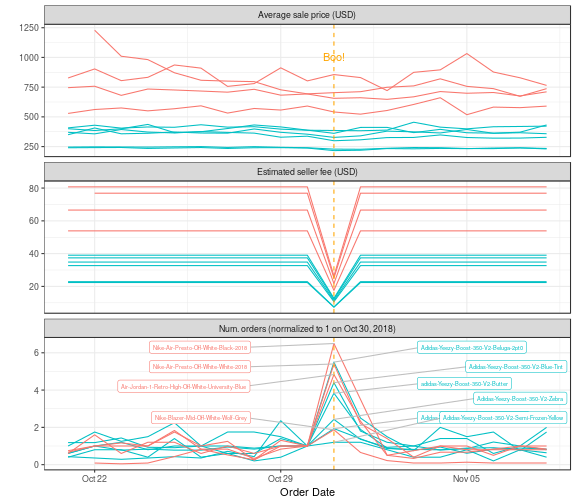
\includegraphics[width = \linewidth]{volume.pdf}
\\
\begin{footnotesize}
\begin{singlespace}
\end{singlespace}
\end{footnotesize}
\end{minipage} 
\end{figure}


\end{document}


